\logg{Torsdag 12. September}{10:00 til 16:00 (6 timer)}{
Møtte opp klokken 09:45 for å delta på oppstartsmøte som skulle starte klokken 10:00. På møtet ble det informert om at alle praksis-studentene skal deles opp inn i forskjellige prosjekter. Deretter blir alle prosjektene presentert; 'research and development', 'digital integration' og 'service and design'.\\

Studentene fikk velge fritt om hvilke av prosjektene de ville delta på. Studenten \textit{Vegard Arnesen Mytting} meldte seg til prosjektet sammen med \textit{Research and Development} avdelingen, sammen med to andre medstudenter. \\

Der får studentene vite at de skal få utdelt arbeids-laptoper, hvor de da skal installere Linux (Ubuntu) som operativsystem. Dette blir startet, og det blir fort oppdaget at dette var utfordrende, ettersom Windows' \textit{Bit Locker} ikke ville tillate Ubuntu. Dette førte oss til å få hjelp av en som jobber på bedriften til å fikse alle laptopene til dem som hadde dette problemet. \\

Etter at Linux ble installert på laptopen, ble det spist lunsj sammen med hele \textit{RnD} gruppen. Der var det brødskiver og en salatbar. \\

Etter lunsjen var det på tide å installere alle programmene man vil trenge til å kunne jobbe. Da måtte man installere \textit{Visual Studio Code}, for å kunne kode og utvikle. \textit{Git} for versjonskontroll og for å kunne hente repositoriet til koden. \textit{Slack} for kommunikasjon mellom gruppen. \textit{Postgresql} for å kunne få tilgang til databasen til prosjektet. \textit{DBeaver} for å kunne bearbeide og arbeide med databasen. \textit{Conda} for å skaffe seg et Python utviklingsmiljø. Til slutt \textit{Docker} for å kunne bygge og teste applikasjonen som skal bli jobbet med.

\begin{figure}[H]
\centering
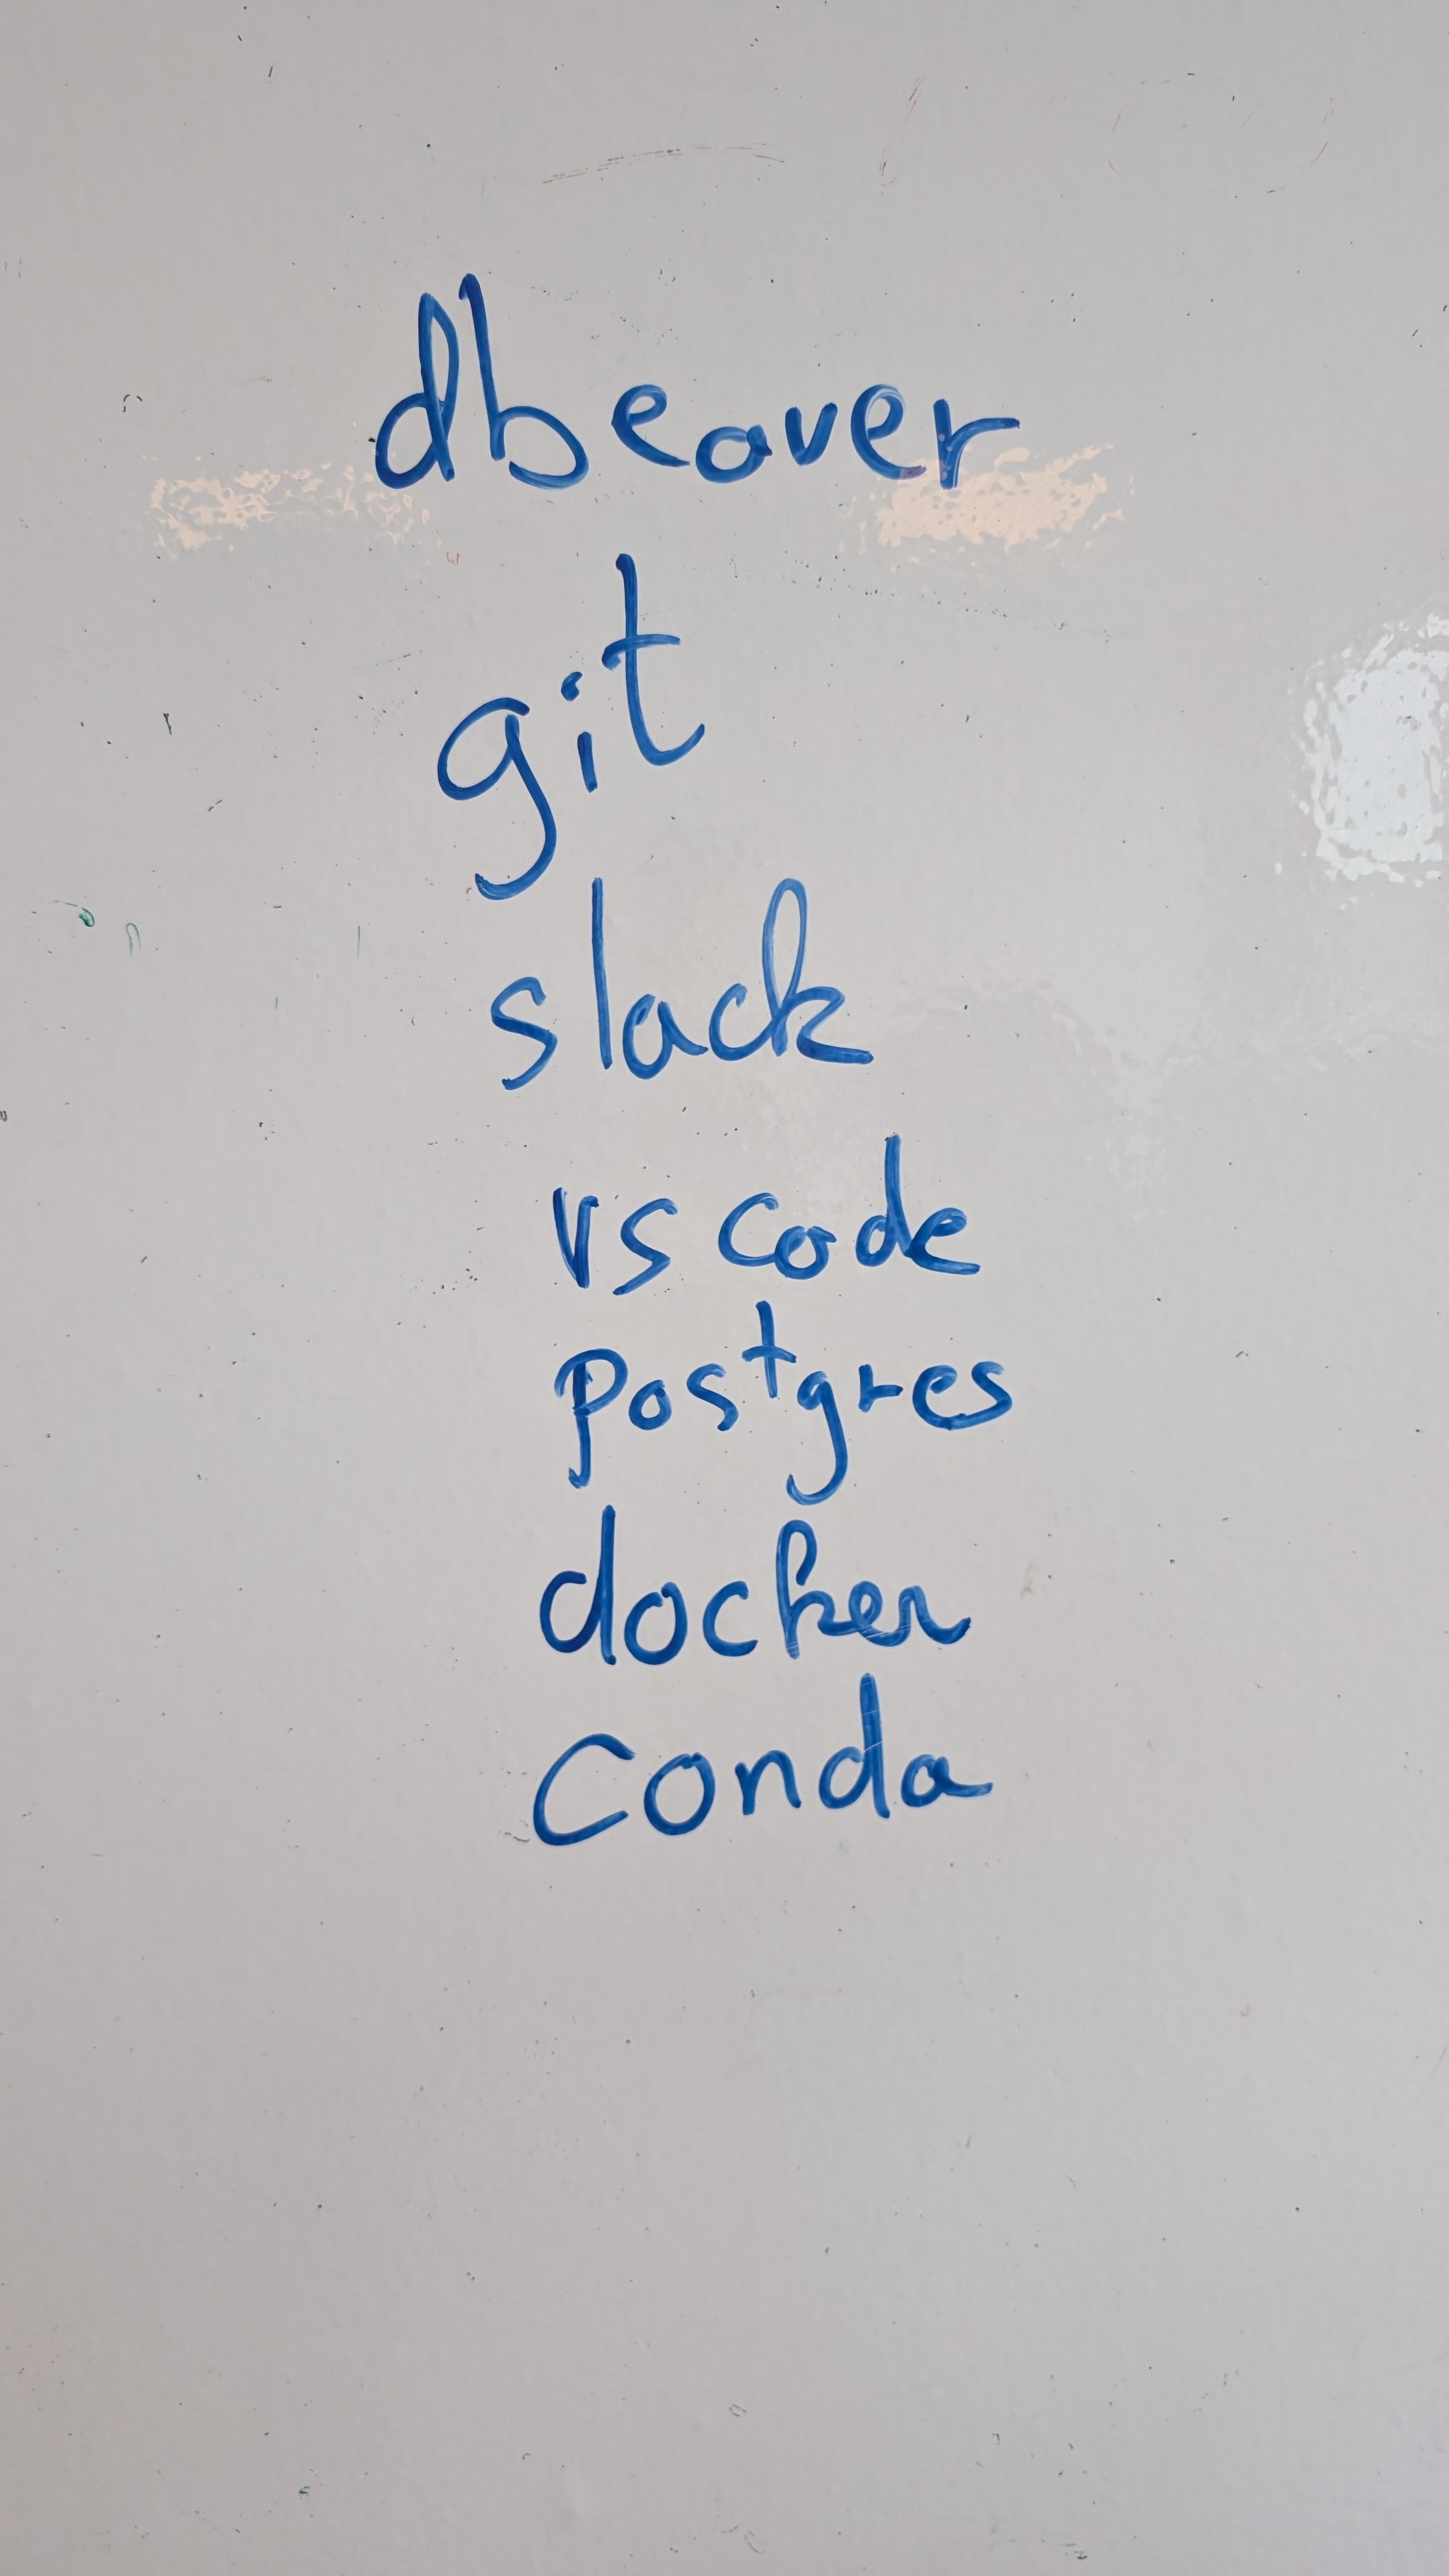
\includegraphics[width=0.25\linewidth]{ukentlige logger/images/uke 1/programs_to_download.jpg}
\caption{\label{fig:downloads}Liste over programmer som skal lastes ned.}
\end{figure}

Det ble noen problemer ved nedlastningen av disse programmene. 

\begin{itemize}
    \item Slack ble lasted ned, men var ikke mulig å åpne. Det ble enig om at studenten skal bruke den nett-baserte versjonen av Slack, dersom det blir behov. 
    \item Visual Studio Code fikk problemer når man skulle begynne å installere \textit{extentions}. Enkelte utvidelser gikk greit, mens andre gjorde det umulig å jobbe i programmet (Programmet kjørte ikke).
\end{itemize}

Etter at alt ble installert var klokken 16:00. Studenten pakket da sammen og dro hjem. 
}\\\\\\